\documentclass[conference]{IEEEtran}
\IEEEoverridecommandlockouts
% The preceding line is only needed to identify funding in the first footnote. If that is unneeded, please comment it out.
\usepackage{cite}
\usepackage{amsmath,amssymb,amsfonts}
\usepackage{algorithmic}
\usepackage{graphicx}
\usepackage{textcomp}
\usepackage{xcolor}
\def\BibTeX{{\rm B\kern-.05em{\sc i\kern-.025em b}\kern-.08em
    T\kern-.1667em\lower.7ex\hbox{E}\kern-.125emX}}
\begin{document}

\title{Perbandingan Arsitektur \textit{Model-View-Intent} (MVI) dan  \textit{Model-View-Controller }(MVC) dalam Pengembangan Perangkat Lunak\\
}

\author{\IEEEauthorblockN{1 Felicia Audrey Emmanuel}
\IEEEauthorblockA{\textit{Jurusan Informatika} \\
\textit{Universitas Pradita}\\
Tangerang Selatan, Indonesia \\
felicia.audrey@student.pradita.ac.id}
\and
\IEEEauthorblockN{2 David Tulus Halomoan Haryanto}
\IEEEauthorblockA{\textit{Jurusan Informatika} \\
\textit{Universitas Pradita}\\
Tangerang Selatan, Indonesia \\
david.tulus@student.pradita.ac.id}
\and
\IEEEauthorblockN{3 Anantaujas Cipta Adinata}
\IEEEauthorblockA{\textit{Jurusan Informatika} \\
\textit{Universitas Pradita}\\
Tangerang Selatan, Indonesia \\
anantaujas.cipta@student.pradita.ac.id}
\and
\IEEEauthorblockN{4 William Kent}
\IEEEauthorblockA{\textit{Jurusan Informatika} \\
\textit{Universitas Pradita}\\
Tangerang Selatan, Indonesia \\
william.kent@student.pradita.ac.id}
\and
\IEEEauthorblockN{5 Michael Christian Yehuda PutraLeytha}
\IEEEauthorblockA{\textit{Jurusan Informatika} \\
\textit{Universitas Pradita}\\
Tangerang Selatan, Indonesia\\
michael.christian.yehuda@student.pradita.ac.id}
}

\maketitle

\begin{abstract}
\end{abstract}

\begin{IEEEkeywords}

\end{IEEEkeywords}

\section{Pendahuluan}
Pola arsitektur sangat penting dalam bidang pengembangan perangkat lunak karena pola tersebut memainkan peran penting dalam menentukan struktur dan perilaku setiap aplikasi. Model View Controller (MVC) dan Model View Intent (MVI) adalah dua paradigma arsitektur terkemuka yang telah diadopsi secara luas dalam beberapa tahun terakhir. Salah satu paradigma ini dikenal sebagai Model View Controller. Membangun solusi perangkat lunak yang terukur, dapat dipelihara, dan efisien dapat dicapai dengan bantuan arsitektur ini, yang menyediakan kerangka kerja terorganisir bagi pengembang. 

Sejak didirikan pada akhir tahun 1970an, MVC telah menjadi komponen yang sangat diperlukan dalam bidang rekayasa perangkat lunak \cite{Hidayat_Surarso_2012}. Akarnya dapat ditelusuri kembali ke Smalltalk. Hal ini dilakukan dengan membagi aplikasi menjadi tiga komponen yang saling berhubungan: Model, yang bertugas mengelola data dan logika bisnis; Tampilan, yang bertugas menyajikan antarmuka pengguna; dan Pengontrol, yang bertindak sebagai perantara antara Model dan View, menangani masukan pengguna dan memperbarui Model sesuai kebutuhan \cite{Chauhan_Kumar_Sethia_Alam_2021}. Memisahkan permasalahan ini satu sama lain akan membantu mendorong modularitas dan membuat pemeliharaan dan pengujian menjadi lebih sederhana. Selain itu, MVI adalah pola arsitektur yang relatif baru yang mendapatkan daya tarik, khususnya dalam konteks pemrograman reaktif dan paradigma fungsional. Hal ini karena MVI merupakan pola yang dikembangkan relatif baru \cite{Mezzalira_2018}. 

MVI menekankan pada kekekalan dan aliran data yang dapat diprediksi di seluruh aplikasi. Fondasinya didasarkan pada prinsip aliran data searah. Model, yang bertanggung jawab untuk mewakili keadaan aplikasi saat ini, Tampilan, yang bertanggung jawab untuk merender antarmuka pengguna berdasarkan keadaan saat ini, dan \textit{Intent}, yang merangkum tindakan pengguna sebagai peristiwa yang tidak dapat diubah yang memicu pembaruan keadaan, adalah tiga inti komponen yang membentuk sistem ini [\cite{Gunawan_Lawi_Adnan_2016}. Melalui penggunaan pendekatan ini, gaya pemrograman yang lebih deklaratif dan dapat diprediksi didorong, yang bermanfaat untuk pengembangan aplikasi yang sangat reaktif dan terukur. Karakteristik kinerja MVC dan MVI terus menjadi topik diskusi dan penyelidikan, meskipun faktanya MVC dan MVI menawarkan keunggulan menarik dalam hal pemeliharaan, skalabilitas, dan pemisahan perhatian. Ada kemungkinan besar bahwa efektivitas pola arsitektur dapat berdampak signifikan terhadap pengalaman pengguna secara keseluruhan, khususnya di lingkungan dengan sumber daya terbatas, seperti perangkat seluler atau browser web \cite{Deacon_2009}. 

Pengembang perangkat lunak sangat perlu memahami dan mengoptimalkan kinerja aplikasi yang dibangun menggunakan pola arsitektur berbeda, itulah sebabnya penelitian bertajuk "Unveiling Efficiency: Analyzing Performance in Model View Controller (MVC) vs MVI (Model View Intent)" sangat penting. Pengembang berada di bawah tekanan yang semakin besar untuk menyediakan perangkat lunak yang tidak hanya berfungsi sesuai harapan namun juga berjalan lancar di semua perangkat dan platform seiring kemajuan teknologi dan ekspektasi pengguna yang semakin meningkat \cite{Khotimah_2016}. Selain itu, lingkungan dengan sumber daya terbatas menjadi semakin umum, terutama dalam konteks aplikasi seluler dan web, yang menyoroti pentingnya penelitian ini. 

Meningkatnya jumlah perangkat seluler dan perangkat \textit{Internet of Things} (IoT) menjadikan pengoptimalan kinerja aplikasi menjadi semakin penting guna memberikan pengalaman pengguna yang lancar sekaligus meminimalkan beban pada sumber daya sistem seperti memori, CPU, dan masa pakai baterai \cite{Anhar_Swari_Aditiawan_2024}. Penelitian ini memberikan wawasan praktis kepada pengembang untuk mengatasi masalah kinerja dan meningkatkan kualitas aplikasi dengan menganalisis metrik kinerja penting seperti daya tanggap, pemanfaatan sumber daya, skalabilitas, dan efisiensi baterai. Selain itu, kemampuan pengujian dan kemampuan debug menjadi lebih penting seiring dengan semakin kompleks dan terhubungnya sistem perangkat lunak \cite{Gunawan_Lawi_Adnan_2016}.


 

\section{Kajian Terkait}
\subsection{MVC}
Desain MVC merupakan salah satu desain yang paling penting dalam bidang ilmu komputer\cite{bucanek2009model}.
\begin{figure}[h]
    \centering
    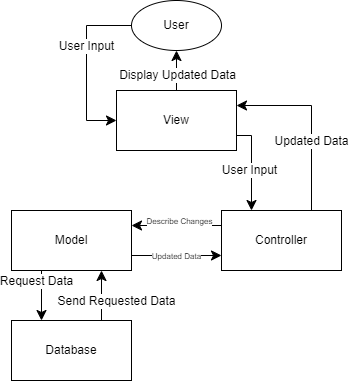
\includegraphics[width = 0.3\textwidth
    ]{images/MVC1.png}
    \caption{Arsitektur MVC}
    \label{fig:enter-label}
\end{figure}

MVC digunakan untuk membagi sebuah aplikasi menjadi tiga bagian, yaitu Model, View, dan Controller \cite{qureshi2014comparison}. Model digunakan untuk pemrosesan data dan hubungan dengan database. Model memberikan data kepada View melalui Controller tanpa mempertimbangkan bagaimana data tersebut dipresentasikan. Bila menerima sebuah notifikasi perubahan atau terjadi sebuah input dari pengguna, Model akan memberi View data yang lebih baru untuk ditampilkan. Tugas Controller adalah untuk menampilkan view berdasarkan input pengguna. Controller menghubungkan Model dengan View. Sebuah input atau pergerakan pada lapisan View akan ditangkap dan diberitakan kepada Controller. Controller akan berinteraksi dengan Model untuk mendapatkan data yang telah diperbaharui dan meneruskan data tersebut pada View. Tugas View adalah untuk menampilkan data tanpa mementingkan proses lain seperti koneksi kepada database. View mempresentasikan data dalam bentuk yang telah diformat dan dapat dibaca oleh pengguna.

MVC berguna untuk sistem yang interaktif, karena memiliki sifat partition-independent, yang berarti bahwa komponen utama dalam MVC dapat beroperasi secara independen satu sama lain, tanpa ada ketergantungan yang kuat di antara mereka. Ini memungkinkan pengembang untuk membuat perubahan tanpa harus khawatir tentang efeknya terhadap komponen yang lain.

MVC, walau bersifat partition-independent, mengalami kesulitan dalam menjalankan proses yang menyebar lapisan pada lokasi yang berbeda, contohnya dengan web application. Pada web application, lapisan View akan berada di device pengguna, namun Controller dan Model bertetap pada server, yang mengakibatkan munculnya permasalahan location-dependant \cite{leff2001web}. Komunikasi pada jaringan, pengiriman data, dan permasalahan dalam sinkronisasi membuat implementasi MVC pada aplikasi berbasis web lebih sulit.


\subsection{MVI}
Arsitektur  MVI,  merupakan  sebuah  arsitektur  yang  menerapkan  aliran  data  searah (unidirectional flow). Model adalah keadaan sebuah aplikasi, yang masih dalam bentuk sebuah data mentah. View adalah representasi keadaan sebuah aplikasi (dari model) yang ditampilkan kepada  pengguna.  Intent  adalah  sebuah  tindakan  yang  dilakukan  sistem  untuk  merespon masukan dari pengguna  dan  perubahan  pada  keadaan  aplikasi  (dari  model). 

\begin{figure}[h]
    \centering
    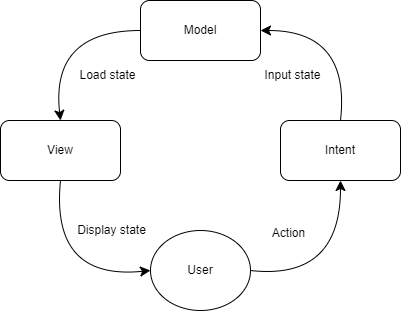
\includegraphics[width = 0.4\textwidth]{images/MVI1.png}
    \caption{Arsitektur MVI}
    \label{fig:enter-label}
\end{figure}

Model-View-Intent, atau MVI, menawarkan banyak kelebihan dan kekurangan dalam pengembangan perangkat lunak perangkat. Salah satu fitur utamanya adalah pemisahan yang jelas antara Model, View, dan Intent, yang membuat kode lebih terstruktur dan lebih mudah digunakan. Dengan aliran data searah, MVI mengurangi risiko bug terkait perubahan tak terduga dan memungkinkan penggunaan status persisten dan berkelanjutan. Selain itu, pendekatan ini memanfaatkan penggunaan logika aplikasi yang stabil, tidak dapat diubah, dan mudah dipahami, sehingga meningkatkan kinerja dan kualitas perangkat lunak. Namun pengguna MVI juga memiliki beberapa kelemahan. Penerapannya seringkali rumit, terutama untuk proyek berukuran kecil atau menengah, dan dapat menimbulkan biaya overhead jika tidak digunakan dengan jujur. Selain itu, terbatasnya ketersediaan sumber daya dan dokumentasi ditambah dengan sifat pendidikan yang berbelit-belit dapat menjadi kendala bagi peserta didik yang belum bias terhadap pendidikan.



\section{Metodologi}
Lorem ipsum dolor sit amet, consectetur adipiscing elit. Aliquam commodo ante ut convallis tincidunt. Nulla id nulla tempor nisl euismod condimentum. Sed finibus lectus lacinia metus luctus ultricies. Fusce eros dolor, dapibus quis sagittis quis, sollicitudin ultrices quam. Integer a feugiat nulla, ac pulvinar nunc. Cras bibendum vehicula enim. Donec sollicitudin porta gravida. Donec sit amet pulvinar augue. Suspendisse porttitor sit amet neque feugiat congue. Curabitur luctus sit amet lectus vel consequat. Sed non sodales enim, sit amet congue metus. Donec nisl eros, aliquam aliquet elementum id, sollicitudin ac neque. Aenean luctus ac dolor eu rhoncus.

Sed libero augue, iaculis sit amet bibendum id, porta nec est. Donec varius arcu nec sem elementum ullamcorper. Pellentesque sed purus sit amet nisl lacinia pulvinar in in leo. Pellentesque gravida iaculis ligula id efficitur. Proin suscipit ultricies diam in fringilla. Nam varius pulvinar dolor id consectetur. Nulla dictum porttitor justo eget dictum. Nullam venenatis eleifend justo a efficitur. Morbi eget sagittis orci. Sed tincidunt ut mauris a rhoncus. Cras posuere tristique massa.

\section{Hasil dan Pembahasan}
Before you begin to format your paper, first write and save the content as a 
separate text file. Complete all content and organizational editing before 
formatting. Please note sections \ref{AA}--\ref{SCM} below for more information on 
proofreading, spelling and grammar.

Keep your text and graphic files separate until after the text has been 
formatted and styled. Do not number text heads---{\LaTeX} will do that 
for you.

\subsection{Abbreviations and Acronyms}\label{AA}
Define abbreviations and acronyms the first time they are used in the text, 
even after they have been defined in the abstract. Abbreviations such as 
IEEE, SI, MKS, CGS, ac, dc, and rms do not have to be defined. Do not use 
abbreviations in the title or heads unless they are unavoidable.

\subsection{Units}
\begin{itemize}
\item Use either SI (MKS) or CGS as primary units. (SI units are encouraged.) English units may be used as secondary units (in parentheses). An exception would be the use of English units as identifiers in trade, such as ``3.5-inch disk drive''.
\item Avoid combining SI and CGS units, such as current in amperes and magnetic field in oersteds. This often leads to confusion because equations do not balance dimensionally. If you must use mixed units, clearly state the units for each quantity that you use in an equation.
\item Do not mix complete spellings and abbreviations of units: ``Wb/m\textsuperscript{2}'' or ``webers per square meter'', not ``webers/m\textsuperscript{2}''. Spell out units when they appear in text: ``. . . a few henries'', not ``. . . a few H''.
\item Use a zero before decimal points: ``0.25'', not ``.25''. Use ``cm\textsuperscript{3}'', not ``cc''.)
\end{itemize}



\subsection{Equations}
Number equations consecutively. To make your 
equations more compact, you may use the solidus (~/~), the exp function, or 
appropriate exponents. Italicize Roman symbols for quantities and variables, 
but not Greek symbols. Use a long dash rather than a hyphen for a minus 
sign. Punctuate equations with commas or periods when they are part of a 
sentence, as in:
\begin{equation}
a+b=\gamma\label{eq}
\end{equation}

Be sure that the 
symbols in your equation have been defined before or immediately following 
the equation. Use ``\eqref{eq}'', not ``Eq.~\eqref{eq}'' or ``equation \eqref{eq}'', except at 
the beginning of a sentence: ``Equation \eqref{eq} is . . .''

\subsection{\LaTeX-Specific Advice}

Please use ``soft'' (e.g., \verb|\eqref{Eq}|) cross references instead
of ``hard'' references (e.g., \verb|(1)|). That will make it possible
to combine sections, add equations, or change the order of figures or
citations without having to go through the file line by line.

Please don't use the \verb|{eqnarray}| equation environment. Use
\verb|{align}| or \verb|{IEEEeqnarray}| instead. The \verb|{eqnarray}|
environment leaves unsightly spaces around relation symbols.

Please note that the \verb|{subequations}| environment in {\LaTeX}
will increment the main equation counter even when there are no
equation numbers displayed. If you forget that, you might write an
article in which the equation numbers skip from (17) to (20), causing
the copy editors to wonder if you've discovered a new method of
counting.

{\BibTeX} does not work by magic. It doesn't get the bibliographic
data from thin air but from .bib files. If you use {\BibTeX} to produce a
bibliography you must send the .bib files. 

{\LaTeX} can't read your mind. If you assign the same label to a
subsubsection and a table, you might find that Table I has been cross
referenced as Table IV-B3. 

{\LaTeX} does not have precognitive abilities. If you put a
\verb|\label| command before the command that updates the counter it's
supposed to be using, the label will pick up the last counter to be
cross referenced instead. In particular, a \verb|\label| command
should not go before the caption of a figure or a table.

Do not use \verb|\nonumber| inside the \verb|{array}| environment. It
will not stop equation numbers inside \verb|{array}| (there won't be
any anyway) and it might stop a wanted equation number in the
surrounding equation.

\subsection{Some Common Mistakes}\label{SCM}
\begin{itemize}
\item The word ``data'' is plural, not singular.
\item The subscript for the permeability of vacuum $\mu_{0}$, and other common scientific constants, is zero with subscript formatting, not a lowercase letter ``o''.
\item In American English, commas, semicolons, periods, question and exclamation marks are located within quotation marks only when a complete thought or name is cited, such as a title or full quotation. When quotation marks are used, instead of a bold or italic typeface, to highlight a word or phrase, punctuation should appear outside of the quotation marks. A parenthetical phrase or statement at the end of a sentence is punctuated outside of the closing parenthesis (like this). (A parenthetical sentence is punctuated within the parentheses.)
\item A graph within a graph is an ``inset'', not an ``insert''. The word alternatively is preferred to the word ``alternately'' (unless you really mean something that alternates).
\item Do not use the word ``essentially'' to mean ``approximately'' or ``effectively''.
\item In your paper title, if the words ``that uses'' can accurately replace the word ``using'', capitalize the ``u''; if not, keep using lower-cased.
\item Be aware of the different meanings of the homophones ``affect'' and ``effect'', ``complement'' and ``compliment'', ``discreet'' and ``discrete'', ``principal'' and ``principle''.
\item Do not confuse ``imply'' and ``infer''.
\item The prefix ``non'' is not a word; it should be joined to the word it modifies, usually without a hyphen.
\item There is no period after the ``et'' in the Latin abbreviation ``et al.''.
\item The abbreviation ``i.e.'' means ``that is'', and the abbreviation ``e.g.'' means ``for example''.
\end{itemize}
An excellent style manual for science writers is \cite{b7}.

\subsection{Authors and Affiliations}
\textbf{The class file is designed for, but not limited to, six authors.} A 
minimum of one author is required for all conference articles. Author names 
should be listed starting from left to right and then moving down to the 
next line. This is the author sequence that will be used in future citations 
and by indexing services. Names should not be listed in columns nor group by 
affiliation. Please keep your affiliations as succinct as possible (for 
example, do not differentiate among departments of the same organization).

\subsection{Identify the Headings}
Headings, or heads, are organizational devices that guide the reader through 
your paper. There are two types: component heads and text heads.

Component heads identify the different components of your paper and are not 
topically subordinate to each other. Examples include Acknowledgments and 
References and, for these, the correct style to use is ``Heading 5''. Use 
``figure caption'' for your Figure captions, and ``table head'' for your 
table title. Run-in heads, such as ``Abstract'', will require you to apply a 
style (in this case, italic) in addition to the style provided by the drop 
down menu to differentiate the head from the text.

Text heads organize the topics on a relational, hierarchical basis. For 
example, the paper title is the primary text head because all subsequent 
material relates and elaborates on this one topic. If there are two or more 
sub-topics, the next level head (uppercase Roman numerals) should be used 
and, conversely, if there are not at least two sub-topics, then no subheads 
should be introduced.

\subsection{Figures and Tables}
\paragraph{Positioning Figures and Tables} Place figures and tables at the top and 
bottom of columns. Avoid placing them in the middle of columns. Large 
figures and tables may span across both columns. Figure captions should be 
below the figures; table heads should appear above the tables. Insert 
figures and tables after they are cited in the text. Use the abbreviation 
``Fig.~\ref{fig}'', even at the beginning of a sentence.

\begin{table}[htbp]
\caption{Table Type Styles}
\begin{center}
\begin{tabular}{|c|c|c|c|}
\hline
\textbf{Table}&\multicolumn{3}{|c|}{\textbf{Table Column Head}} \\
\cline{2-4} 
\textbf{Head} & \textbf{\textit{Table column subhead}}& \textbf{\textit{Subhead}}& \textbf{\textit{Subhead}} \\
\hline
copy& More table copy$^{\mathrm{a}}$& &  \\
\hline
\multicolumn{4}{l}{$^{\mathrm{a}}$Sample of a Table footnote.}
\end{tabular}
\label{tab1}
\end{center}
\end{table}

Figure Labels: Use 8 point Times New Roman for Figure labels. Use words 
rather than symbols or abbreviations when writing Figure axis labels to 
avoid confusing the reader. As an example, write the quantity 
``Magnetization'', or ``Magnetization, M'', not just ``M''. If including 
units in the label, present them within parentheses. Do not label axes only 
with units. In the example, write ``Magnetization (A/m)'' or ``Magnetization 
\{A[m(1)]\}'', not just ``A/m''. Do not label axes with a ratio of 
quantities and units. For example, write ``Temperature (K)'', not 
``Temperature/K''.

\section{Kesimpulan}
\section*{}
\bibliographystyle{plain}
\bibliography{mybib}

\end{document}
